\documentclass{article}\usepackage[]{graphicx}\usepackage[]{color}
%% maxwidth is the original width if it is less than linewidth
%% otherwise use linewidth (to make sure the graphics do not exceed the margin)
\makeatletter
\def\maxwidth{ %
  \ifdim\Gin@nat@width>\linewidth
    \linewidth
  \else
    \Gin@nat@width
  \fi
}
\makeatother

\definecolor{fgcolor}{rgb}{0.345, 0.345, 0.345}
\newcommand{\hlnum}[1]{\textcolor[rgb]{0.686,0.059,0.569}{#1}}%
\newcommand{\hlstr}[1]{\textcolor[rgb]{0.192,0.494,0.8}{#1}}%
\newcommand{\hlcom}[1]{\textcolor[rgb]{0.678,0.584,0.686}{\textit{#1}}}%
\newcommand{\hlopt}[1]{\textcolor[rgb]{0,0,0}{#1}}%
\newcommand{\hlstd}[1]{\textcolor[rgb]{0.345,0.345,0.345}{#1}}%
\newcommand{\hlkwa}[1]{\textcolor[rgb]{0.161,0.373,0.58}{\textbf{#1}}}%
\newcommand{\hlkwb}[1]{\textcolor[rgb]{0.69,0.353,0.396}{#1}}%
\newcommand{\hlkwc}[1]{\textcolor[rgb]{0.333,0.667,0.333}{#1}}%
\newcommand{\hlkwd}[1]{\textcolor[rgb]{0.737,0.353,0.396}{\textbf{#1}}}%
\let\hlipl\hlkwb

\usepackage{framed}
\makeatletter
\newenvironment{kframe}{%
 \def\at@end@of@kframe{}%
 \ifinner\ifhmode%
  \def\at@end@of@kframe{\end{minipage}}%
  \begin{minipage}{\columnwidth}%
 \fi\fi%
 \def\FrameCommand##1{\hskip\@totalleftmargin \hskip-\fboxsep
 \colorbox{shadecolor}{##1}\hskip-\fboxsep
     % There is no \\@totalrightmargin, so:
     \hskip-\linewidth \hskip-\@totalleftmargin \hskip\columnwidth}%
 \MakeFramed {\advance\hsize-\width
   \@totalleftmargin\z@ \linewidth\hsize
   \@setminipage}}%
 {\par\unskip\endMakeFramed%
 \at@end@of@kframe}
\makeatother

\definecolor{shadecolor}{rgb}{.97, .97, .97}
\definecolor{messagecolor}{rgb}{0, 0, 0}
\definecolor{warningcolor}{rgb}{1, 0, 1}
\definecolor{errorcolor}{rgb}{1, 0, 0}
\newenvironment{knitrout}{}{} % an empty environment to be redefined in TeX

\usepackage{alltt}
\title{Problem Set 4}
\author{Cameron Adams}


\usepackage{float, hyperref}
\usepackage[margin = 1in]{geometry}
\usepackage{graphicx}
\usepackage{sectsty}
\usepackage{hyperref}
\IfFileExists{upquote.sty}{\usepackage{upquote}}{}
\begin{document}
%\SweaveOpts{concordance=TRUE}

\maketitle






\section{In class we discussed the idea of a closure as a function ...}


\begin{knitrout}
\definecolor{shadecolor}{rgb}{0.969, 0.969, 0.969}\color{fgcolor}\begin{kframe}
\begin{alltt}
\hlstd{x} \hlkwb{<-} \hlnum{1}\hlopt{:}\hlnum{10}

\hlstd{f} \hlkwb{<-} \hlkwa{function}\hlstd{(}\hlkwc{input}\hlstd{)\{}
    \hlstd{data} \hlkwb{<-} \hlstd{input}
    \hlstd{g} \hlkwb{<-} \hlkwa{function}\hlstd{(}\hlkwc{param}\hlstd{)} \hlkwd{return}\hlstd{(param} \hlopt{*} \hlstd{data)}
    \hlkwd{return}\hlstd{(g)}
\hlstd{\}}

\hlstd{myFun} \hlkwb{<-} \hlkwd{f}\hlstd{(x)}
\hlstd{data} \hlkwb{<-} \hlnum{100}
\hlkwd{myFun}\hlstd{(}\hlnum{3}\hlstd{)}
\end{alltt}
\begin{verbatim}
##  [1]  3  6  9 12 15 18 21 24 27 30
\end{verbatim}
\begin{alltt}
\hlstd{x} \hlkwb{<-} \hlnum{100}
\hlkwd{myFun}\hlstd{(}\hlnum{3}\hlstd{)}
\end{alltt}
\begin{verbatim}
##  [1]  3  6  9 12 15 18 21 24 27 30
\end{verbatim}
\end{kframe}
\end{knitrout}

\subsection{What is the maximum number of copies that exist of the vector 1:10 during the first execution of myFun()? Why?} %1a

There are two copies of x, one in global memory from \texttt{x <- 1:10}, one in local memory of the function \texttt{myFun()}.

\subsection{Use serialize() to generate a sequence of bytes that store  ...} %1b

\begin{knitrout}
\definecolor{shadecolor}{rgb}{0.969, 0.969, 0.969}\color{fgcolor}\begin{kframe}
\begin{alltt}
\hlstd{x} \hlkwb{<-} \hlnum{1}\hlopt{:}\hlnum{1e6}
\hlstd{x_size} \hlkwb{<-} \hlkwd{object_size}\hlstd{(x)}
\hlstd{x_len} \hlkwb{<-} \hlkwd{length}\hlstd{(}\hlkwd{serialize}\hlstd{(x,} \hlkwa{NULL}\hlstd{))} \hlcom{#62}


\hlstd{f} \hlkwb{<-} \hlkwa{function}\hlstd{(}\hlkwc{input}\hlstd{)\{}
    \hlstd{data} \hlkwb{<-} \hlstd{input}
    \hlstd{g} \hlkwb{<-} \hlkwa{function}\hlstd{(}\hlkwc{param}\hlstd{)} \hlkwd{return}\hlstd{(param} \hlopt{*} \hlstd{data)}
    \hlkwd{return}\hlstd{(g)}
\hlstd{\}}
\hlstd{myFun} \hlkwb{<-} \hlkwd{f}\hlstd{(x)}
\hlkwd{rm}\hlstd{(x)}

\hlstd{myFun_size} \hlkwb{<-} \hlkwd{object.size}\hlstd{(myFun)}
\hlstd{myFun_len} \hlkwb{<-} \hlkwd{length}\hlstd{(}\hlkwd{serialize}\hlstd{(myFun,} \hlkwa{NULL}\hlstd{))}
\hlstd{myFun_len;x_len}
\end{alltt}
\begin{verbatim}
## [1] 8010067
## [1] 4000022
\end{verbatim}
\begin{alltt}
\hlstd{myFun_len}\hlopt{-}\hlstd{x_len}
\end{alltt}
\begin{verbatim}
## [1] 4010045
\end{verbatim}
\begin{alltt}
\hlstd{x_size;myFun_size}
\end{alltt}
\begin{verbatim}
## 4 MB
## 1560 bytes
\end{verbatim}
\end{kframe}
\end{knitrout}

No, the size of the serialized object is not what I expect. it seems that there are two copies of \texttt{x} inside of \texttt{myFun}, plus one copy of x in the compiled code of \texttt{myFun}. Therefore there are three copies, which is weird because from 1a) we know there should be two.

\subsection{It seems unnecessary to have the "data <- input" line ...} %1c


\begin{knitrout}
\definecolor{shadecolor}{rgb}{0.969, 0.969, 0.969}\color{fgcolor}\begin{kframe}
\begin{alltt}
\hlstd{x} \hlkwb{<-} \hlnum{1}\hlopt{:}\hlnum{10}     \hlcom{#set vector 1:10 to object x                  }

\hlstd{f} \hlkwb{<-} \hlkwa{function}\hlstd{(}\hlkwc{data}\hlstd{)\{}
    \hlstd{g} \hlkwb{<-} \hlkwa{function}\hlstd{(}\hlkwc{param}\hlstd{)} \hlkwd{return}\hlstd{(param} \hlopt{*} \hlstd{data)}
    \hlkwd{return}\hlstd{(g)}
\hlstd{\}}

\hlstd{myFun} \hlkwb{<-} \hlkwd{f}\hlstd{(x)}
\hlkwd{rm}\hlstd{(x)}
\hlstd{data} \hlkwb{<-} \hlnum{100}
\hlkwd{myFun}\hlstd{(}\hlnum{3}\hlstd{)}
\end{alltt}


{\ttfamily\noindent\bfseries\color{errorcolor}{\#\# Error in myFun(3): object 'x' not found}}\end{kframe}
\end{knitrout}

When \texttt{myFun <- f(x)} is evaluated, \texttt{f(x)} is assigned to \texttt{myFun}, the function \texttt{f} with value \texttt{x} is not evaluated; a promise is created for evaluation of \texttt{f(x)} and it will be lazy-evaluated. That occures when \texttt{myFun()} is evaluate with input. Since we are removing \texttt{x} from memory before evaluate \texttt{myFun}, we get an error.

\subsection{Can you figure out a way to make the code in part (c) work ...} %1d

\begin{knitrout}
\definecolor{shadecolor}{rgb}{0.969, 0.969, 0.969}\color{fgcolor}\begin{kframe}
\begin{alltt}
\hlstd{x} \hlkwb{<-} \hlnum{1}\hlopt{:}\hlnum{10}
\hlkwd{length}\hlstd{(}\hlkwd{serialize}\hlstd{(x,} \hlkwa{NULL}\hlstd{))}
\end{alltt}
\begin{verbatim}
## [1] 62
\end{verbatim}
\begin{alltt}
\hlstd{f} \hlkwb{<-} \hlkwa{function}\hlstd{(}\hlkwc{data}\hlstd{)\{}
    \hlkwd{invisible}\hlstd{(}\hlkwd{is.numeric}\hlstd{(data))}
    \hlstd{g} \hlkwb{<-} \hlkwa{function}\hlstd{(}\hlkwc{param}\hlstd{)} \hlkwd{return}\hlstd{(param} \hlopt{*} \hlstd{data)}
    \hlkwd{return}\hlstd{(g)}
\hlstd{\}}

\hlstd{myFun} \hlkwb{<-} \hlkwd{f}\hlstd{(x)}
\hlkwd{rm}\hlstd{(x)}
\hlstd{data} \hlkwb{<-} \hlnum{100}
\hlkwd{myFun}\hlstd{(}\hlnum{3}\hlstd{)}
\end{alltt}
\begin{verbatim}
##  [1]  3  6  9 12 15 18 21 24 27 30
\end{verbatim}
\begin{alltt}
\hlkwd{length}\hlstd{(}\hlkwd{serialize}\hlstd{(myFun,} \hlkwa{NULL}\hlstd{))}
\end{alltt}
\begin{verbatim}
## [1] 9458
\end{verbatim}
\begin{alltt}
\hlkwd{length}\hlstd{(}\hlkwd{serialize}\hlstd{(}\hlnum{1}\hlopt{:}\hlnum{10}\hlstd{,} \hlkwa{NULL}\hlstd{))}
\end{alltt}
\begin{verbatim}
## [1] 62
\end{verbatim}
\end{kframe}
\end{knitrout}

We can make part(c) work by somehow inserting the intput data into the \texttt{f()} closure itself. Invisibily testing whether the data is of class numeric does that and allows the code work to work. Another way to do it would be to simply put the data input into the function.
\begin{knitrout}
\definecolor{shadecolor}{rgb}{0.969, 0.969, 0.969}\color{fgcolor}\begin{kframe}
\begin{alltt}
\hlstd{x} \hlkwb{<-} \hlnum{1}\hlopt{:}\hlnum{10}
\hlkwd{length}\hlstd{(}\hlkwd{serialize}\hlstd{(x,} \hlkwa{NULL}\hlstd{))}
\end{alltt}
\begin{verbatim}
## [1] 62
\end{verbatim}
\begin{alltt}
\hlstd{f} \hlkwb{<-} \hlkwa{function}\hlstd{(}\hlkwc{data}\hlstd{)\{}
    \hlstd{data}
    \hlstd{g} \hlkwb{<-} \hlkwa{function}\hlstd{(}\hlkwc{param}\hlstd{)} \hlkwd{return}\hlstd{(param} \hlopt{*} \hlstd{data)}
    \hlkwd{return}\hlstd{(g)}
\hlstd{\}}
\end{alltt}
\end{kframe}
\end{knitrout}


\section{This question explores memory use and copying with lists. In answering this question you can ignore what is happening with the list attributes, which are also reported by .Internal(inspect()).} %2

****************
\textbf{For all problem 2 questions: RStudio doesn't work for these problems. Code and output for these answers are from sessions run in standalone R.}
****************

\subsection{Consider a list of vectors. Modify an element of one of the vectors. Can R make the change in place, without creating a new list or a new vector?} %2a


\begin{knitrout}
\definecolor{shadecolor}{rgb}{0.969, 0.969, 0.969}\color{fgcolor}\begin{kframe}
\begin{alltt}
\hlkwd{rm}(list=\hlkwd{ls}())

\hlcom{#create list of random numbers, 10 elements, 5 list elements and inspect}
vecList <-\hlkwd{lapply}(1:5,\hlkwd{function}(x) \hlkwd{sample}(1:100,10))
\hlkwd{class}(vecList)
[1] \hlstr{"list"}
\hlkwd{length}(vecList)
[1] 5
\hlkwd{.Internal}(\hlkwd{inspect}(vecList))
@7fa06fd6f010 19 VECSXP g1c4 [MARK,\hlkwd{NAM}(1)] (len=5, tl=0)
  @7fa070765950 13 INTSXP g1c4 [MARK] (len=10, tl=0) 74,36,19,24,34,...
  @7fa07201fee0 13 INTSXP g0c4 [] (len=10, tl=0) 10,59,61,67,70,...
  @7fa0720201b8 13 INTSXP g0c4 [] (len=10, tl=0) 78,12,11,79,13,...
  @7fa0720202f0 13 INTSXP g0c4 [] (len=10, tl=0) 52,45,36,50,67,...
  @7fa072018cd8 13 INTSXP g0c4 [] (len=10, tl=0) 42,34,64,14,37,...

\hlcom{#change value of 1st element in 1st list element and inspect}
vecList[[1]][1] <- 10
\hlkwd{.Internal}(\hlkwd{inspect}(vecList))
@7fa06fd6f010 19 VECSXP g1c4 [MARK,\hlkwd{NAM}(1)] (len=5, tl=0)
  @7fa0718966a8 14 REALSXP g0c5 [] (len=10, tl=0) 10,36,19,24,34,...
  @7fa07201fee0 13 INTSXP g0c4 [] (len=10, tl=0) 10,59,61,67,70,...
  @7fa0720201b8 13 INTSXP g0c4 [] (len=10, tl=0) 78,12,11,79,13,...
  @7fa0720202f0 13 INTSXP g0c4 [] (len=10, tl=0) 52,45,36,50,67,...
  @7fa072018cd8 13 INTSXP g0c4 [] (len=10, tl=0) 42,34,64,14,37,...
\end{alltt}
\end{kframe}
\end{knitrout}





R \textit{cannot} modify an element of one of the vectors without making a copy of the vector that changed and pointing to the new vector memory address.

\subsection{Next, make a copy of the list and determine ...?} %2b

\begin{knitrout}
\definecolor{shadecolor}{rgb}{0.969, 0.969, 0.969}\color{fgcolor}\begin{kframe}
\begin{alltt}
vecListCopy <- vecList
\hlkwd{.Internal}(\hlkwd{inspect}(vecList))
@7f8b7eb3ed50 19 VECSXP g1c4 [MARK,\hlkwd{NAM}(2)] (len=5, tl=0)
  @7f8b7ed25f48 14 REALSXP g0c5 [] (len=10, tl=0) 10,47,11,60,80,...
  @7f8b7ee52478 13 INTSXP g0c4 [] (len=10, tl=0) 55,33,67,16,53,...
  @7f8b7ee527b8 13 INTSXP g0c4 [] (len=10, tl=0) 4,8,51,30,24,...
  @7f8b7ee4e540 13 INTSXP g0c4 [] (len=10, tl=0) 6,12,48,93,54,...
  @7f8b7ee4e818 13 INTSXP g0c4 [] (len=10, tl=0) 47,95,13,59,81,...
\hlkwd{.Internal}(\hlkwd{inspect}(vecListCopy))
@7f8b7eb3ed50 19 VECSXP g1c4 [MARK,\hlkwd{NAM}(2)] (len=5, tl=0)
  @7f8b7ed25f48 14 REALSXP g0c5 [] (len=10, tl=0) 10,47,11,60,80,...
  @7f8b7ee52478 13 INTSXP g0c4 [] (len=10, tl=0) 55,33,67,16,53,...
  @7f8b7ee527b8 13 INTSXP g0c4 [] (len=10, tl=0) 4,8,51,30,24,...
  @7f8b7ee4e540 13 INTSXP g0c4 [] (len=10, tl=0) 6,12,48,93,54,...
  @7f8b7ee4e818 13 INTSXP g0c4 [] (len=10, tl=0) 47,95,13,59,81,...

vecListCopy[[1]][1] <- 99
\hlkwd{.Internal}(\hlkwd{inspect}(vecListCopy))
@7f8b7ee4e9b8 19 VECSXP g0c4 [\hlkwd{NAM}(1)] (len=5, tl=0)
  @7f8b7ed25ff0 14 REALSXP g0c5 [] (len=10, tl=0) 99,47,11,60,80,...
  @7f8b7ee52478 13 INTSXP g0c4 [\hlkwd{NAM}(2)] (len=10, tl=0) 55,33,67,16,53,...
  @7f8b7ee527b8 13 INTSXP g0c4 [\hlkwd{NAM}(2)] (len=10, tl=0) 4,8,51,30,24,...
  @7f8b7ee4e540 13 INTSXP g0c4 [\hlkwd{NAM}(2)] (len=10, tl=0) 6,12,48,93,54,...
  @7f8b7ee4e818 13 INTSXP g0c4 [\hlkwd{NAM}(2)] (len=10, tl=0) 47,95,13,59,81,...
\end{alltt}
\end{kframe}
\end{knitrout}

When a copy of the list is made, the copy points to address of teh original list. When an element is changed in one of teh vectors in the list copy, the address copied list now has a new address, and the vector with a changed element has a new address. The unchanged vectors in the copied have the same memory addess as in the original list. 

\subsection{Now make a list of lists ...} %2c

\begin{knitrout}
\definecolor{shadecolor}{rgb}{0.969, 0.969, 0.969}\color{fgcolor}\begin{kframe}
\begin{alltt}
listOfLists <-\hlkwd{lapply}(1:2, 
+                      \hlkwd{function}(x) \hlkwd{lapply}(1:2,
+                                         \hlkwd{function}(x) \hlkwd{sample}(1:100,10)))
\hlkwd{length}(listOfLists)
[1] 2
\hlkwd{length}(listOfLists[[1]])
[1] 2

\hlcom{#Copy the list}
listOfListsCopy <- listOfLists
\hlkwd{.Internal}(\hlkwd{inspect}(listOfLists))
@7fdb504304e0 19 VECSXP g1c2 [MARK,\hlkwd{NAM}(2)] (len=2, tl=0)
  @7fdb50430550 19 VECSXP g1c2 [MARK,\hlkwd{NAM}(1)] (len=2, tl=0)
    @7fdb5079b810 13 INTSXP g1c4 [MARK] (len=10, tl=0) 66,47,11,60,80,...
    @7fdb5079b6d8 13 INTSXP g1c4 [MARK] (len=10, tl=0) 55,33,67,16,53,...
  @7fdb5227c578 19 VECSXP g0c2 [] (len=2, tl=0)
    @7fdb52231618 13 INTSXP g0c4 [] (len=10, tl=0) 4,8,51,30,24,...
    @7fdb511bc270 13 INTSXP g0c4 [] (len=10, tl=0) 6,12,48,93,54,...
\hlkwd{.Internal}(\hlkwd{inspect}(listOfListsCopy))
@7fdb504304e0 19 VECSXP g1c2 [MARK,\hlkwd{NAM}(2)] (len=2, tl=0)
  @7fdb50430550 19 VECSXP g1c2 [MARK,\hlkwd{NAM}(1)] (len=2, tl=0)
    @7fdb5079b810 13 INTSXP g1c4 [MARK] (len=10, tl=0) 66,47,11,60,80,...
    @7fdb5079b6d8 13 INTSXP g1c4 [MARK] (len=10, tl=0) 55,33,67,16,53,...
  @7fdb5227c578 19 VECSXP g0c2 [] (len=2, tl=0)
    @7fdb52231618 13 INTSXP g0c4 [] (len=10, tl=0) 4,8,51,30,24,...
    @7fdb511bc270 13 INTSXP g0c4 [] (len=10, tl=0) 6,12,48,93,54,...

\hlcom{#Add an element to the second list}
listOfListsCopy[[2]][[3]] <- 99:90
\hlkwd{.Internal}(\hlkwd{inspect}(listOfListsCopy))
@7fdb52278278 19 VECSXP g0c2 [\hlkwd{NAM}(1)] (len=2, tl=0)
  @7fdb50430550 19 VECSXP g1c2 [MARK,\hlkwd{NAM}(2)] (len=2, tl=0)
    @7fdb5079b810 13 INTSXP g1c4 [MARK] (len=10, tl=0) 66,47,11,60,80,...
    @7fdb5079b6d8 13 INTSXP g1c4 [MARK] (len=10, tl=0) 55,33,67,16,53,...
  @7fdb5117fdf0 19 VECSXP g0c3 [] (len=3, tl=0)
    @7fdb52231618 13 INTSXP g0c4 [\hlkwd{NAM}(2)] (len=10, tl=0) 4,8,51,30,24,...
    @7fdb511bc270 13 INTSXP g0c4 [\hlkwd{NAM}(2)] (len=10, tl=0) 6,12,48,93,54,...
    @7fdb511bc340 13 INTSXP g0c4 [\hlkwd{NAM}(1)] (len=10, tl=0) 99,98,97,96,95,...
\end{alltt}
\end{kframe}
\end{knitrout}

The following is shared between the two lists (\texttt{listOfLists, listOfListsCopy}):
\begin{itemize}
    \item First list of list, \texttt{listOfListsCopy[[1]][[1]]} and \texttt{listOfLists[[1]][[1]]}.
    \item The first two vectors of the second list have the same address and were not copied, \texttt{listOfLists[[2]][[1]] == listOfListsCopy[[2]][[1]]} and \texttt{listOfLists[[2]][[2]] == listOfListsCopy[[2]][[2]]}.
\end{itemize}
Everything else was copied and is not shared between lists.

\subsection{Run the following code in a new R session ...} %2d

\begin{knitrout}
\definecolor{shadecolor}{rgb}{0.969, 0.969, 0.969}\color{fgcolor}\begin{kframe}
\begin{alltt}
\hlkwd{gc}()
         \hlkwd{used} (Mb) gc \hlkwd{trigger} (Mb) max \hlkwd{used} (Mb)
Ncells 257840 13.8     460000 24.6   350000 18.7
Vcells 537163  4.1    1023718  7.9   911750  7.0

tmp <- \hlkwd{list}()
x <- \hlkwd{rnorm}(1e7)
tmp[[1]] <- x
tmp[[2]] <- x

\hlkwd{.Internal}(\hlkwd{inspect}(tmp))
@7fced1c59008 19 VECSXP g0c2 [\hlkwd{NAM}(1)] (len=2, tl=0)
  @11235a000 14 REALSXP g0c7 [\hlkwd{NAM}(2)] (len=10000000, tl=0) 0.401138,-1.2158,0.950013,2.19382,0.43482,...
  @11235a000 14 REALSXP g0c7 [\hlkwd{NAM}(2)] (len=10000000, tl=0) 0.401138,-1.2158,0.950013,2.19382,0.43482,...

\hlkwd{object.size}(tmp)
160000136 bytes

\hlkwd{gc}()
           \hlkwd{used} (Mb) gc \hlkwd{trigger}  (Mb) max \hlkwd{used} (Mb)
Ncells   258528 13.9     592000  31.7   350000 18.7
Vcells 10538593 80.5   15576004 118.9 10545243 80.5
\end{alltt}
\end{kframe}
\end{knitrout}
The help file for \texttt{object.size()} specifically says that the function "does not detect if elements of a list are shared". The function is simply adding up the memory usage of each element, without taking duplciate addresses into account.

\section{Challenge 5 of Section 7.3 of Unit 4. The following is real code...} %3

\begin{knitrout}
\definecolor{shadecolor}{rgb}{0.969, 0.969, 0.969}\color{fgcolor}\begin{kframe}
\begin{alltt}
\hlkwd{rm}\hlstd{(}\hlkwc{list}\hlstd{=}\hlkwd{ls}\hlstd{())}

\hlkwd{setwd}\hlstd{(}\hlstr{"/Users/CamAdams/repos/STAT243/ps4/"}\hlstd{)}

\hlkwd{load}\hlstd{(}\hlstr{'ps4prob3.Rda'}\hlstd{)} \hlcom{# should have A, n, K}

\hlcom{################----------------------------------------------------------------}
\hlcom{## Student's version of the function}

\hlstd{ll} \hlkwb{<-} \hlkwa{function}\hlstd{(}\hlkwc{Theta}\hlstd{,} \hlkwc{A}\hlstd{) \{}
    \hlstd{sum.ind} \hlkwb{<-} \hlkwd{which}\hlstd{(A}\hlopt{==}\hlnum{1}\hlstd{,} \hlkwc{arr.ind}\hlstd{=T)}
    \hlstd{logLik} \hlkwb{<-} \hlkwd{sum}\hlstd{(}\hlkwd{log}\hlstd{(Theta[sum.ind]))} \hlopt{-} \hlkwd{sum}\hlstd{(Theta)}
    \hlkwd{return}\hlstd{(logLik)}
\hlstd{\}}

\hlstd{oneUpdate} \hlkwb{<-} \hlkwa{function}\hlstd{(}\hlkwc{A}\hlstd{,} \hlkwc{n}\hlstd{,} \hlkwc{K}\hlstd{,} \hlkwc{theta.old}\hlstd{,} \hlkwc{thresh} \hlstd{=} \hlnum{0.1}\hlstd{) \{}
    \hlstd{theta.old1} \hlkwb{<-} \hlstd{theta.old}
    \hlstd{Theta.old} \hlkwb{<-} \hlstd{theta.old} \hlopt \hlkwd{t}\hlstd{(theta.old)}
    \hlstd{L.old} \hlkwb{<-} \hlkwd{ll}\hlstd{(Theta.old, A)}
    \hlstd{q} \hlkwb{<-} \hlkwd{array}\hlstd{(}\hlnum{0}\hlstd{,} \hlkwc{dim} \hlstd{=} \hlkwd{c}\hlstd{(n, n, K))}
    \hlkwa{for} \hlstd{(i} \hlkwa{in} \hlnum{1}\hlopt{:}\hlstd{n) \{}
        \hlkwa{for} \hlstd{(j} \hlkwa{in} \hlnum{1}\hlopt{:}\hlstd{n) \{}
            \hlkwa{for} \hlstd{(z} \hlkwa{in} \hlnum{1}\hlopt{:}\hlstd{K) \{}
                \hlkwa{if} \hlstd{(theta.old[i, z]}\hlopt{*}\hlstd{theta.old[j, z]} \hlopt{==} \hlnum{0}\hlstd{)\{}
                    \hlstd{q[i, j, z]} \hlkwb{<-} \hlnum{0}
                    \hlstd{\}} \hlkwa{else} \hlstd{\{}
                        \hlstd{q[i, j, z]} \hlkwb{<-} \hlstd{theta.old[i, z]}\hlopt{*}\hlstd{theta.old[j, z]} \hlopt{/}
                            \hlstd{Theta.old[i, j]}
                    \hlstd{\}}
            \hlstd{\}}
        \hlstd{\}}
    \hlstd{\}}


    \hlstd{theta.new} \hlkwb{<-} \hlstd{theta.old}
    \hlkwa{for} \hlstd{(z} \hlkwa{in} \hlnum{1}\hlopt{:}\hlstd{K) \{}
        \hlstd{theta.new[,z]} \hlkwb{<-} \hlkwd{rowSums}\hlstd{(A}\hlopt{*}\hlstd{q[,,z])}\hlopt{/}\hlkwd{sqrt}\hlstd{(}\hlkwd{sum}\hlstd{(A}\hlopt{*}\hlstd{q[,,z]))}
    \hlstd{\}}

    \hlstd{Theta.new} \hlkwb{<-} \hlstd{theta.new} \hlopt \hlkwd{t}\hlstd{(theta.new)}
    \hlstd{L.new} \hlkwb{<-} \hlkwd{ll}\hlstd{(Theta.new, A)}
    \hlstd{converge.check} \hlkwb{<-} \hlkwd{abs}\hlstd{(L.new} \hlopt{-} \hlstd{L.old)} \hlopt{<} \hlstd{thresh}
    \hlstd{theta.new} \hlkwb{<-} \hlstd{theta.new}\hlopt{/}\hlkwd{rowSums}\hlstd{(theta.new)}
    \hlkwd{return}\hlstd{(}\hlkwd{list}\hlstd{(}\hlkwc{theta} \hlstd{= theta.new,} \hlkwc{loglik} \hlstd{= L.new,}
                \hlkwc{converged} \hlstd{= converge.check))}
\hlstd{\}}

\hlcom{# initialize the parameters at random starting values}
\hlstd{temp} \hlkwb{<-} \hlkwd{matrix}\hlstd{(}\hlkwd{runif}\hlstd{(n}\hlopt{*}\hlstd{K), n, K)}
\hlstd{theta.init} \hlkwb{<-} \hlstd{temp}\hlopt{/}\hlkwd{rowSums}\hlstd{(temp)}

\hlcom{################----------------------------------------------------------------}
\hlcom{## My version of the function}

\hlstd{llMe} \hlkwb{<-} \hlkwa{function}\hlstd{(}\hlkwc{Theta}\hlstd{,} \hlkwc{A}\hlstd{) \{}

    \hlcom{#calculate loglikelihood}
    \hlstd{logLik} \hlkwb{<-} \hlkwd{sum}\hlstd{(}\hlkwd{log}\hlstd{(Theta[}\hlkwd{which}\hlstd{(A}\hlopt{==}\hlnum{1}\hlstd{,} \hlkwc{arr.ind}\hlstd{=T)]))} \hlopt{-} \hlkwd{sum}\hlstd{(Theta)}

    \hlkwd{return}\hlstd{(logLik)}
\hlstd{\}}

\hlstd{oneUpdateMe} \hlkwb{<-} \hlkwa{function}\hlstd{(}\hlkwc{A}\hlstd{,} \hlkwc{n}\hlstd{,} \hlkwc{K}\hlstd{,} \hlkwc{theta.old}\hlstd{,} \hlkwc{thresh} \hlstd{=} \hlnum{0.1}\hlstd{) \{}

    \hlstd{Theta.old} \hlkwb{<-} \hlkwd{tcrossprod}\hlstd{(theta.old)}
    \hlstd{L.old} \hlkwb{<-} \hlkwd{llMe}\hlstd{(Theta.old, A)}

    \hlstd{Theta.new} \hlkwb{<-} \hlkwd{tcrossprod}\hlstd{(}
                    \hlkwd{sapply}\hlstd{(}\hlnum{1}\hlopt{:}\hlstd{K,} \hlkwa{function}\hlstd{(}\hlkwc{z}\hlstd{) \{}
                        \hlstd{q_z} \hlkwb{<-} \hlkwd{matrix}\hlstd{(theta.old[ , z]} \hlopt \hlkwd{t}\hlstd{(theta.old[ , z]),}
                                        \hlkwc{ncol} \hlstd{= n)} \hlopt{/}
                                        \hlstd{Theta.old}
                    \hlkwd{return}\hlstd{(}\hlkwd{rowSums}\hlstd{(A} \hlopt{*} \hlstd{q_z)} \hlopt{/} \hlkwd{sqrt}\hlstd{(}\hlkwd{sum}\hlstd{(A} \hlopt{*} \hlstd{q_z)))}
                        \hlstd{\}))}

    \hlstd{L.new} \hlkwb{<-} \hlkwd{llMe}\hlstd{(Theta.new, A)}

    \hlkwd{return}\hlstd{(}\hlkwd{list}\hlstd{(}\hlkwc{theta} \hlstd{= theta.old,} \hlkwc{loglik} \hlstd{= L.new,}
                \hlkwc{converged} \hlstd{=} \hlnum{FALSE}\hlstd{))}
\hlstd{\}}

\hlstd{oneUpdateMe2} \hlkwb{<-} \hlkwa{function}\hlstd{(}\hlkwc{A}\hlstd{,} \hlkwc{n}\hlstd{,} \hlkwc{K}\hlstd{,} \hlkwc{theta.old}\hlstd{,} \hlkwc{thresh} \hlstd{=} \hlnum{0.1}\hlstd{) \{}

    \hlstd{theta.old} \hlkwb{<-} \hlstd{theta.init}
    \hlstd{Theta.old} \hlkwb{<-} \hlkwd{tcrossprod}\hlstd{(theta.old)}
    \hlstd{L.old} \hlkwb{<-} \hlkwd{llMe}\hlstd{(Theta.old, A)}

    \hlcom{#Theta.new <- tcrossprod(}
    \hlcom{#                sapply(1:K, function(z) \{}
    \hlcom{#                    q_z <- matrix(theta.old[ , z] %o% t(theta.old[ , z]), }
    \hlcom{#                                    ncol = n) /}
    \hlcom{#                                    Theta.old}
    \hlcom{#                    return(rowSums(A * q_z) / sqrt(sum(A * q_z)))}
    \hlcom{#                    \}))}

    \hlstd{Theta.new} \hlkwb{<-} \hlkwd{tcrossprod}\hlstd{(}
                    \hlkwd{vapply}\hlstd{(}\hlnum{1}\hlopt{:}\hlstd{K,} \hlkwc{FUN.VALUE} \hlstd{=} \hlkwd{numeric}\hlstd{(}\hlnum{500}\hlstd{),} \hlkwa{function}\hlstd{(}\hlkwc{z}\hlstd{) \{}
                        \hlstd{q_z} \hlkwb{<-} \hlkwd{matrix}\hlstd{(theta.old[ , z]} \hlopt \hlkwd{t}\hlstd{(theta.old[ , z]),}
                                        \hlkwc{ncol} \hlstd{= n)} \hlopt{/}
                                        \hlstd{Theta.old}
                        \hlkwd{return}\hlstd{(}\hlkwd{rowSums}\hlstd{(A} \hlopt{*} \hlstd{q_z)} \hlopt{/} \hlkwd{sqrt}\hlstd{(}\hlkwd{sum}\hlstd{(A} \hlopt{*} \hlstd{q_z)))}
                        \hlstd{\}))}


    \hlstd{q_z} \hlkwb{<-} \hlkwd{vapply}\hlstd{(}\hlnum{1}\hlopt{:}\hlstd{K,} \hlkwc{FUN.VALUE} \hlstd{=} \hlkwd{numeric}\hlstd{(}\hlnum{250000}\hlstd{),} \hlkwa{function}\hlstd{(}\hlkwc{z}\hlstd{) \{}
                        \hlkwd{matrix}\hlstd{(theta.old[ , z]} \hlopt \hlkwd{t}\hlstd{(theta.old[ , z]),}
                                        \hlkwc{ncol} \hlstd{= n)} \hlopt{/}
                                        \hlstd{Theta.old\})}
            \hlkwd{vapply}\hlstd{(}\hlnum{1}\hlopt{:}\hlstd{K )}

    \hlstd{L.new} \hlkwb{<-} \hlkwd{llMe}\hlstd{(Theta.new, A)}

    \hlkwd{return}\hlstd{(}\hlkwd{list}\hlstd{(}\hlkwc{theta} \hlstd{= theta.old,} \hlkwc{loglik} \hlstd{= L.new,}
                \hlkwc{converged} \hlstd{=} \hlnum{FALSE}\hlstd{))}
\hlstd{\}}

\hlcom{# initialize the parameters at random starting values}
\hlstd{temp} \hlkwb{<-} \hlkwd{matrix}\hlstd{(}\hlkwd{runif}\hlstd{(n} \hlopt{*} \hlstd{K), n, K)}
\hlstd{theta.init} \hlkwb{<-} \hlstd{temp}\hlopt{/}\hlkwd{rowSums}\hlstd{(temp)}

\hlcom{# benchmark student version vs. my version}
\hlkwd{require}\hlstd{(microbenchmark)}
\hlkwd{microbenchmark}\hlstd{(out} \hlkwb{<-} \hlkwd{oneUpdate}\hlstd{(A, n, K, theta.init),}      \hlcom{#student's verions}
               \hlstd{outMe} \hlkwb{<-} \hlkwd{oneUpdateMe}\hlstd{(A, n, K, theta.init),}  \hlcom{#my version}
               \hlkwc{times} \hlstd{=} \hlnum{20L}\hlstd{,} \hlkwc{unit} \hlstd{=} \hlstr{"s"}\hlstd{)}            \hlcom{#avg. over 20 iterations}
\end{alltt}
\begin{verbatim}
## Unit: seconds
##                                       expr       min       lq     mean
##      out <- oneUpdate(A, n, K, theta.init) 8.3034210 8.615452 9.025107
##  outMe <- oneUpdateMe(A, n, K, theta.init) 0.7965409 0.867914 1.001540
##     median       uq      max neval
##  8.8505975 9.592912 10.03484    20
##  0.9279685 1.013755  1.65792    20
\end{verbatim}
\begin{alltt}
\hlkwd{microbenchmark}\hlstd{(out} \hlkwb{<-} \hlkwd{oneUpdateMe}\hlstd{(A, n, K, theta.init),}      \hlcom{#student's verions}
               \hlstd{outMe} \hlkwb{<-} \hlkwd{oneUpdateMe2}\hlstd{(A, n, K, theta.init),}  \hlcom{#my version}
               \hlkwc{times} \hlstd{=} \hlnum{20L}\hlstd{,} \hlkwc{unit} \hlstd{=} \hlstr{"s"}\hlstd{)}
\end{alltt}


{\ttfamily\noindent\bfseries\color{errorcolor}{\#\# Error in match.fun(FUN): argument "{}FUN"{} is missing, with no default}}\begin{alltt}
\hlcom{#check to see if loglik values match between versions}
\hlstd{out}\hlopt{$}\hlstd{loglik}
\end{alltt}
\begin{verbatim}
## [1] -41666.03
\end{verbatim}
\begin{alltt}
\hlstd{out}\hlopt{$}\hlstd{loglik} \hlopt{==} \hlstd{outMe}\hlopt{$}\hlstd{loglik}
\end{alltt}
\begin{verbatim}
## [1] TRUE
\end{verbatim}
\end{kframe}
\end{knitrout}

My code changes:

\begin{itemize}
    \item Removed: \texttt{theta.old1 <- theta.old}
    \item Removed: \texttt{q <- array(0, dim = c(n, n, K))}
    \item \texttt{crossprod(theta.old)} instead of \texttt{theta.old \%*\% t(theta.old)}
    \item Combined calculating array \texttt{q} with for loops and \texttt{Theta.new} into one \texttt{sapply()} indexing through \texttt{z}-dimension.
\end{itemize}

With these changes, I was able to speed up the liklihood function by about a factor of 10. Further improvements might be made with use of \texttt{vapply} instead of \texttt{sapply}, but I ran out of time to implement.

\section{} %4
\subsection{This is a variation on Challenge 8 in Section 7.3 of Unit 4. The goal is to write a function to sample k values without replacement ...}  %4a

\begin{knitrout}
\definecolor{shadecolor}{rgb}{0.969, 0.969, 0.969}\color{fgcolor}\begin{kframe}
\begin{alltt}
\hlkwd{rm}\hlstd{(}\hlkwc{list}\hlstd{=}\hlkwd{ls}\hlstd{())}

\hlcom{################}
\hlcom{#PIKK methods}

\hlcom{#defualt}
\hlstd{PIKK} \hlkwb{<-} \hlkwa{function}\hlstd{(}\hlkwc{x}\hlstd{,} \hlkwc{k}\hlstd{) \{}

    \hlstd{x[}\hlkwd{sort}\hlstd{(}\hlkwd{runif}\hlstd{(}\hlkwd{length}\hlstd{(x)),} \hlkwc{index.return} \hlstd{=} \hlnum{TRUE}\hlstd{)}\hlopt{$}\hlstd{ix[}\hlnum{1}\hlopt{:}\hlstd{k]]}

\hlstd{\}}

\hlcom{#my first method}
\hlstd{PIKK.me1} \hlkwb{<-} \hlkwa{function}\hlstd{(}\hlkwc{x}\hlstd{,} \hlkwc{k}\hlstd{) \{}

    \hlkwd{unique}\hlstd{(x[}\hlkwd{as.integer}\hlstd{(}\hlkwd{runif}\hlstd{(k} \hlopt{*} \hlnum{1.1}\hlstd{,} \hlkwc{min} \hlstd{=} \hlnum{1}\hlstd{,} \hlkwc{max} \hlstd{=} \hlkwd{length}\hlstd{(x)))])[}\hlnum{1}\hlopt{:}\hlstd{k]}

\hlstd{\}}

\hlcom{#my second method}
\hlstd{PIKK.me2} \hlkwb{<-} \hlkwa{function}\hlstd{(}\hlkwc{x}\hlstd{,} \hlkwc{k}\hlstd{) \{}

    \hlkwd{unique}\hlstd{(}\hlkwd{as.integer}\hlstd{(}\hlkwd{runif}\hlstd{(k} \hlopt{*} \hlnum{1.1}\hlstd{,} \hlkwc{min} \hlstd{=} \hlnum{1}\hlstd{,} \hlkwc{max} \hlstd{=} \hlkwd{length}\hlstd{(x))))[}\hlnum{1}\hlopt{:}\hlstd{k]}

\hlstd{\}}

\hlcom{############}
\hlcom{# test that PIKK methods}
\hlkwd{require}\hlstd{(testthat)}

\hlcom{#test paramters}
\hlstd{x} \hlkwb{<-} \hlnum{1}\hlopt{:}\hlnum{10000}
\hlstd{k} \hlkwb{<-} \hlkwd{length}\hlstd{(x)} \hlopt{*} \hlnum{0.05}

\hlcom{#run test code}
\hlstd{PIKK.out} \hlkwb{<-} \hlkwd{PIKK}\hlstd{(x, k)}
\hlstd{PIKK.me1.out} \hlkwb{<-} \hlkwd{PIKK.me1}\hlstd{(x, k)}
\hlstd{PIKK.me2.out} \hlkwb{<-} \hlkwd{PIKK.me2}\hlstd{(x, k)}

\hlcom{#view output}
\hlkwd{head}\hlstd{(PIKK.out)}
\end{alltt}
\begin{verbatim}
## [1] 2151 7621 1881 2265 2078 5140
\end{verbatim}
\begin{alltt}
\hlkwd{head}\hlstd{(PIKK.me1.out)}
\end{alltt}
\begin{verbatim}
## [1] 6886 2782 6776 5779 5264 4758
\end{verbatim}
\begin{alltt}
\hlkwd{head}\hlstd{(PIKK.me2.out)}
\end{alltt}
\begin{verbatim}
## [1] 8179 9103 6495 1497  100 9537
\end{verbatim}
\begin{alltt}
\hlcom{#testing function}
\hlkwd{test_that}\hlstd{(}\hlstr{"Output is an integer vector of length(k)"}\hlstd{, \{}

    \hlkwd{expect_that}\hlstd{(PIKK.out,} \hlkwd{is_a}\hlstd{(}\hlstr{"integer"}\hlstd{))}        \hlcom{#is integer}
    \hlkwd{expect_that}\hlstd{(PIKK.me1.out,} \hlkwd{is_a}\hlstd{(}\hlstr{"integer"}\hlstd{))}    \hlcom{#is integer}
    \hlkwd{expect_that}\hlstd{(PIKK.me2.out,} \hlkwd{is_a}\hlstd{(}\hlstr{"integer"}\hlstd{))}    \hlcom{#is integer}

    \hlkwd{expect_equal}\hlstd{(} \hlkwd{length}\hlstd{(PIKK.out), k)}             \hlcom{#length==k}

    \hlkwd{expect_equal}\hlstd{(}\hlkwd{length}\hlstd{(PIKK.out),}                 \hlcom{#output lengths match}
                 \hlkwd{length}\hlstd{(PIKK.me1.out),}
                 \hlkwd{length}\hlstd{(PIKK.me2.out)}
                \hlstd{)}
\hlstd{\})}

\hlcom{##############}
\hlcom{#Benchmark sampling methods}

\hlcom{#wrapper function}
\hlstd{benchMeanWrapper} \hlkwb{<-} \hlkwa{function}\hlstd{(}\hlkwc{...}\hlstd{,} \hlkwc{n}\hlstd{,} \hlkwc{k}\hlstd{,} \hlkwc{times}\hlstd{,} \hlkwc{units}\hlstd{) \{}

    \hlstd{x} \hlkwb{<-} \hlnum{1}\hlopt{:}\hlstd{n}   \hlcom{#set vector to sample from}

    \hlstd{expr} \hlkwb{<-} \hlkwd{list}\hlstd{(}\hlkwd{paste}\hlstd{(...,} \hlkwc{sep} \hlstd{=} \hlstr{","}\hlstd{))} \hlcom{#get list expressions}

    \hlcom{#create benchmark expression}
    \hlstd{benchExpr} \hlkwb{<-} \hlkwd{paste}\hlstd{(}\hlstr{"microbenchmark("}\hlstd{, expr,}
                       \hlstr{", times = times,"}\hlstd{,} \hlstr{"unit = units)"}\hlstd{)}

    \hlcom{#eval benchmark expressions}
    \hlstd{bench} \hlkwb{<-} \hlkwd{eval}\hlstd{(}\hlkwd{parse}\hlstd{(}\hlkwc{text} \hlstd{= benchExpr))}

    \hlcom{#return mean of iterations}
    \hlkwd{return}\hlstd{(}\hlkwd{summary}\hlstd{(bench)}\hlopt{$}\hlstd{mean)}

\hlstd{\}}

\hlcom{#benchmark expressions with different n and k values and }
\hlstd{n} \hlkwb{<-} \hlkwd{c}\hlstd{(}\hlnum{1e3}\hlstd{,} \hlnum{1e4}\hlstd{,} \hlnum{1e5}\hlstd{,} \hlnum{1e6}\hlstd{,} \hlnum{1e7}\hlstd{)}
\hlstd{kn_ratio} \hlkwb{<-} \hlkwd{c}\hlstd{(}\hlnum{0.05}\hlstd{,} \hlnum{0.25}\hlstd{,} \hlnum{0.5}\hlstd{,} \hlnum{0.75}\hlstd{)}

\hlcom{# k:n=1:20}
\hlstd{bench_5pp} \hlkwb{<-} \hlkwd{mapply}\hlstd{(}\hlstr{"PIKK(x, k)"}\hlstd{,} \hlstr{"PIKK.me1(x, k)"}\hlstd{,}
                    \hlstr{"PIKK.me2(x, k)"}\hlstd{,} \hlstr{"sample(x, k)"}\hlstd{,}
                    \hlkwc{n} \hlstd{= n,} \hlkwc{k} \hlstd{= n} \hlopt{*} \hlstd{kn_ratio[}\hlnum{1}\hlstd{],} \hlkwc{times} \hlstd{=} \hlnum{20L}\hlstd{,} \hlkwc{units} \hlstd{=} \hlstr{"ms"}\hlstd{,}
                    \hlkwc{FUN} \hlstd{= benchMeanWrapper,} \hlkwc{SIMPLIFY} \hlstd{= T)}

\hlcom{# k:n=1:4}
\hlstd{bench_25pp} \hlkwb{<-} \hlkwd{mapply}\hlstd{(}\hlstr{"PIKK(x, k)"}\hlstd{,} \hlstr{"PIKK.me1(x, k)"}\hlstd{,}
                    \hlstr{"PIKK.me2(x, k)"}\hlstd{,} \hlstr{"sample(x, k)"}\hlstd{,}
                    \hlkwc{n} \hlstd{= n,} \hlkwc{k} \hlstd{= n} \hlopt{*} \hlstd{kn_ratio[}\hlnum{2}\hlstd{],} \hlkwc{times} \hlstd{=} \hlnum{20L}\hlstd{,} \hlkwc{units} \hlstd{=} \hlstr{"ms"}\hlstd{,}
                    \hlkwc{FUN} \hlstd{= benchMeanWrapper,} \hlkwc{SIMPLIFY} \hlstd{= T)}

\hlcom{# k:n=1:2}
\hlstd{bench_50pp} \hlkwb{<-} \hlkwd{mapply}\hlstd{(}\hlstr{"PIKK(x, k)"}\hlstd{,} \hlstr{"PIKK.me1(x, k)"}\hlstd{,}
                    \hlstr{"PIKK.me2(x, k)"}\hlstd{,} \hlstr{"sample(x, k)"}\hlstd{,}
                    \hlkwc{n} \hlstd{= n,} \hlkwc{k} \hlstd{= n} \hlopt{*} \hlstd{kn_ratio[}\hlnum{3}\hlstd{],} \hlkwc{times} \hlstd{=} \hlnum{20L}\hlstd{,} \hlkwc{units} \hlstd{=} \hlstr{"ms"}\hlstd{,}
                    \hlkwc{FUN} \hlstd{= benchMeanWrapper,} \hlkwc{SIMPLIFY} \hlstd{= T)}

\hlcom{# k:n=3:4}
\hlstd{bench_75pp} \hlkwb{<-} \hlkwd{mapply}\hlstd{(}\hlstr{"PIKK(x, k)"}\hlstd{,} \hlstr{"PIKK.me1(x, k)"}\hlstd{,}
                    \hlstr{"PIKK.me2(x, k)"}\hlstd{,} \hlstr{"sample(x, k)"}\hlstd{,}
                    \hlkwc{n} \hlstd{= n,} \hlkwc{k} \hlstd{= n} \hlopt{*} \hlstd{kn_ratio[}\hlnum{4}\hlstd{],} \hlkwc{times} \hlstd{=} \hlnum{20L}\hlstd{,} \hlkwc{units} \hlstd{=} \hlstr{"ms"}\hlstd{,}
                    \hlkwc{FUN} \hlstd{= benchMeanWrapper,} \hlkwc{SIMPLIFY} \hlstd{= T)}
\end{alltt}
\end{kframe}
\end{knitrout}


\begin{kframe}
\begin{alltt}
\hlcom{###############}
\hlcom{#create table output}

\hlkwd{options}\hlstd{(}\hlkwc{scipen} \hlstd{=} \hlopt{-}\hlnum{1}\hlstd{)} \hlcom{#set for printing in sci notatation.}

\hlcom{#create dataframe of benchmarks}
\hlstd{bench_Combined} \hlkwb{<-} \hlkwd{data.frame}\hlstd{(}
                    \hlkwd{cbind}\hlstd{(}\hlkwd{as.character}\hlstd{(}\hlkwd{rep}\hlstd{(n,} \hlkwd{length}\hlstd{(kn_ratio))),}
                            \hlkwd{sort}\hlstd{(}\hlkwd{as.character}\hlstd{(}\hlkwd{rep}\hlstd{(kn_ratio,} \hlkwd{length}\hlstd{(n)))),}
                            \hlkwc{row.names} \hlstd{=} \hlkwa{NULL}\hlstd{),}
                        \hlkwd{rbind}\hlstd{(}\hlkwd{t}\hlstd{(bench_5pp),} \hlkwd{t}\hlstd{(bench_25pp),}
                                \hlkwd{t}\hlstd{(bench_50pp),} \hlkwd{t}\hlstd{(bench_75pp)),} \hlkwc{row.names} \hlstd{=} \hlkwa{NULL}\hlstd{)}

\hlkwd{colnames}\hlstd{(bench_Combined)} \hlkwb{<-} \hlkwd{c}\hlstd{(}\hlstr{"n"}\hlstd{,} \hlstr{"kn_ratio"}\hlstd{,} \hlstr{"PIKK"}\hlstd{,} \hlstr{"PIKK.me1"}\hlstd{,}
                              \hlstr{"PIKK.me2"}\hlstd{,} \hlstr{"sample()"}\hlstd{)}

\hlcom{#sort on kn_ratio}
\hlstd{bench_Combined} \hlkwb{<-} \hlstd{bench_Combined[}\hlkwd{order}\hlstd{(bench_Combined}\hlopt{$}\hlstd{n), ]}

\hlcom{#print table}
\hlkwd{require}\hlstd{(xtable)}
\hlstd{tbl} \hlkwb{<-} \hlkwd{xtable}\hlstd{(bench_Combined,}
              \hlkwc{caption} \hlstd{=} \hlstr{"Average runtime for sampling functions"}\hlstd{,}
              \hlkwc{comment} \hlstd{= F,} \hlkwc{align} \hlstd{=} \hlkwd{c}\hlstd{(}\hlstr{"c"}\hlstd{,} \hlstr{"c|"}\hlstd{,}\hlstr{"c|"}\hlstd{,}\hlkwd{rep}\hlstd{(}\hlstr{"c"}\hlstd{,} \hlnum{4}\hlstd{)),}
              \hlkwc{digits} \hlstd{=} \hlnum{3}\hlstd{)}
\hlkwd{print}\hlstd{(tbl,} \hlkwc{floating} \hlstd{= T,} \hlkwc{table.placement} \hlstd{=} \hlstr{"H"}\hlstd{,} \hlkwc{comment} \hlstd{= F,}
      \hlkwc{include.rownames} \hlstd{= F,} \hlkwc{caption.placement} \hlstd{=} \hlstr{"top"}\hlstd{,} \hlkwc{caption.width} \hlstd{=} \hlstr{"35em"}\hlstd{,}
      \hlkwc{hline.after} \hlstd{=} \hlkwd{c}\hlstd{(}\hlopt{-}\hlnum{1}\hlstd{,} \hlkwd{seq}\hlstd{(}\hlnum{0}\hlstd{,} \hlnum{20}\hlstd{,} \hlnum{4}\hlstd{)))}
\end{alltt}
\end{kframe}\begin{table}[H]
\centering
\parbox{35em}{\caption{Average runtime for sampling functions}} 
\begin{tabular}{c|c|cccc}
  \hline
n & kn\_ratio & PIKK & PIKK.me1 & PIKK.me2 & sample() \\ 
  \hline
1000 & 0.05 & 0.303 & 0.207 & 0.191 & 0.010 \\ 
  1000 & 0.25 & 0.363 & 0.117 & 0.290 & 0.058 \\ 
  1000 & 0.5 & 0.256 & 0.103 & 0.096 & 0.030 \\ 
  1000 & 0.75 & 0.217 & 0.119 & 0.101 & 0.038 \\ 
   \hline
1e+04 & 0.05 & 1.267 & 0.063 & 0.047 & 0.025 \\ 
  1e+04 & 0.25 & 2.703 & 0.527 & 0.480 & 0.159 \\ 
  1e+04 & 0.5 & 2.102 & 0.807 & 0.794 & 0.227 \\ 
  1e+04 & 0.75 & 1.710 & 1.087 & 0.921 & 0.249 \\ 
   \hline
1e+05 & 0.05 & 14.927 & 0.562 & 0.639 & 0.440 \\ 
  1e+05 & 0.25 & 18.113 & 5.965 & 5.117 & 1.805 \\ 
  1e+05 & 0.5 & 19.101 & 13.074 & 11.095 & 2.813 \\ 
  1e+05 & 0.75 & 14.279 & 14.279 & 11.470 & 2.695 \\ 
   \hline
1e+06 & 0.05 & 212.277 & 6.388 & 5.064 & 10.229 \\ 
  1e+06 & 0.25 & 225.024 & 48.401 & 33.390 & 24.907 \\ 
  1e+06 & 0.5 & 228.619 & 129.356 & 91.190 & 54.773 \\ 
  1e+06 & 0.75 & 194.788 & 129.295 & 116.454 & 42.718 \\ 
   \hline
1e+07 & 0.05 & 2073.781 & 111.529 & 68.122 & 99.461 \\ 
  1e+07 & 0.25 & 2046.066 & 440.257 & 353.139 & 293.116 \\ 
  1e+07 & 0.5 & 2072.891 & 973.011 & 822.627 & 548.917 \\ 
  1e+07 & 0.75 & 2110.236 & 1455.055 & 1229.538 & 702.065 \\ 
   \hline
\end{tabular}
\end{table}




\begin{knitrout}
\definecolor{shadecolor}{rgb}{0.969, 0.969, 0.969}\color{fgcolor}\begin{kframe}
\begin{alltt}
\hlcom{###############}
\hlcom{#create plots}

\hlcom{#0.05}
\hlkwd{par}\hlstd{(}\hlkwc{mfrow} \hlstd{=} \hlkwd{c}\hlstd{(}\hlnum{1}\hlstd{,} \hlnum{5}\hlstd{),} \hlkwc{mar} \hlstd{=} \hlkwd{c}\hlstd{(}\hlnum{3}\hlstd{,}\hlnum{1}\hlstd{,}\hlnum{4}\hlstd{,}\hlnum{1}\hlstd{),} \hlkwc{oma} \hlstd{=} \hlkwd{c}\hlstd{(}\hlnum{2}\hlstd{,} \hlnum{5}\hlstd{,} \hlnum{2}\hlstd{,} \hlnum{0}\hlstd{))}
\hlkwa{for} \hlstd{(i} \hlkwa{in} \hlnum{1}\hlopt{:}\hlnum{5}\hlstd{) \{}
    \hlkwd{barplot}\hlstd{(bench_5pp[ , i],}  \hlkwc{horiz} \hlstd{= T,}
            \hlkwc{ylab} \hlstd{=} \hlstr{""}\hlstd{,}
            \hlkwc{main} \hlstd{=} \hlkwd{paste0}\hlstd{(}\hlstr{"n = "}\hlstd{, n[i],} \hlstr{",\textbackslash{}n k = "}\hlstd{, n[i]}\hlopt{*}\hlnum{0.05}\hlstd{),}
            \hlkwc{las} \hlstd{=} \hlnum{1}\hlstd{,} \hlkwc{cex.names} \hlstd{=} \hlnum{1}\hlstd{,}
            \hlkwc{names.arg} \hlstd{=} \hlkwa{if}\hlstd{(i}\hlopt{==}\hlnum{1}\hlstd{) \{}\hlkwd{c}\hlstd{(}\hlstr{"PIKK"}\hlstd{,} \hlstr{"PIKK.me1"}\hlstd{,}
                              \hlstr{"PIKK.me2"}\hlstd{,} \hlstr{"sample()"}\hlstd{)\}}
            \hlkwa{else} \hlstd{\{}\hlstr{" "}\hlstd{\})}
\hlstd{\}}
\hlkwd{mtext}\hlstd{(}\hlstr{"Comparison of sampling functions k:n = 1:20"}\hlstd{,}
      \hlkwc{side} \hlstd{=} \hlnum{3}\hlstd{,} \hlkwc{outer} \hlstd{= T,} \hlkwc{font} \hlstd{=} \hlnum{2}\hlstd{)}
\hlkwd{mtext}\hlstd{(}\hlstr{"Mean(millseconds), 20 iterations "}\hlstd{,}
      \hlkwc{side} \hlstd{=} \hlnum{1}\hlstd{,} \hlkwc{outer} \hlstd{= T,} \hlkwc{font} \hlstd{=} \hlnum{1}\hlstd{,} \hlkwc{cex} \hlstd{=} \hlnum{0.75}\hlstd{)}

\hlcom{#0.25}
\hlkwd{par}\hlstd{(}\hlkwc{mfrow} \hlstd{=} \hlkwd{c}\hlstd{(}\hlnum{1}\hlstd{,} \hlnum{5}\hlstd{),} \hlkwc{mar} \hlstd{=} \hlkwd{c}\hlstd{(}\hlnum{3}\hlstd{,}\hlnum{1}\hlstd{,}\hlnum{4}\hlstd{,}\hlnum{1}\hlstd{),} \hlkwc{oma} \hlstd{=} \hlkwd{c}\hlstd{(}\hlnum{2}\hlstd{,} \hlnum{5}\hlstd{,} \hlnum{2}\hlstd{,} \hlnum{0}\hlstd{))}
\hlkwa{for} \hlstd{(i} \hlkwa{in} \hlnum{1}\hlopt{:}\hlnum{5}\hlstd{) \{}
    \hlkwd{barplot}\hlstd{(bench_25pp[ , i],}  \hlkwc{horiz} \hlstd{= T,}
            \hlkwc{ylab} \hlstd{=} \hlstr{""}\hlstd{,}
            \hlkwc{main} \hlstd{=} \hlkwd{paste0}\hlstd{(}\hlstr{"n = "}\hlstd{, n[i],} \hlstr{",\textbackslash{}n k = "}\hlstd{, n[i]} \hlopt{*} \hlnum{0.25}\hlstd{),}
            \hlkwc{las} \hlstd{=} \hlnum{1}\hlstd{,} \hlkwc{cex.names} \hlstd{=} \hlnum{1}\hlstd{,}
            \hlkwc{names.arg} \hlstd{=} \hlkwa{if}\hlstd{(i}\hlopt{==}\hlnum{1}\hlstd{) \{}\hlkwd{c}\hlstd{(}\hlstr{"PIKK"}\hlstd{,} \hlstr{"PIKK.me1"}\hlstd{,}
                              \hlstr{"PIKK.me2"}\hlstd{,} \hlstr{"sample()"}\hlstd{)\}}
            \hlkwa{else} \hlstd{\{}\hlstr{" "}\hlstd{\})}
\hlstd{\}}
\hlkwd{mtext}\hlstd{(}\hlstr{"Comparison of sampling functions k:n = 1:4"}\hlstd{,}
      \hlkwc{side} \hlstd{=} \hlnum{3}\hlstd{,} \hlkwc{outer} \hlstd{= T,} \hlkwc{font} \hlstd{=} \hlnum{2}\hlstd{)}
\hlkwd{mtext}\hlstd{(}\hlstr{"Mean(millseconds), 20 iterations "}\hlstd{,}
      \hlkwc{side} \hlstd{=} \hlnum{1}\hlstd{,} \hlkwc{outer} \hlstd{= T,} \hlkwc{font} \hlstd{=} \hlnum{1}\hlstd{,} \hlkwc{cex} \hlstd{=} \hlnum{0.75}\hlstd{)}

\hlcom{#0.50}
\hlkwd{par}\hlstd{(}\hlkwc{mfrow} \hlstd{=} \hlkwd{c}\hlstd{(}\hlnum{1}\hlstd{,} \hlnum{5}\hlstd{),} \hlkwc{mar} \hlstd{=} \hlkwd{c}\hlstd{(}\hlnum{3}\hlstd{,}\hlnum{1}\hlstd{,}\hlnum{4}\hlstd{,}\hlnum{1}\hlstd{),} \hlkwc{oma} \hlstd{=} \hlkwd{c}\hlstd{(}\hlnum{2}\hlstd{,} \hlnum{5}\hlstd{,} \hlnum{2}\hlstd{,} \hlnum{0}\hlstd{))}
\hlkwa{for} \hlstd{(i} \hlkwa{in} \hlnum{1}\hlopt{:}\hlnum{5}\hlstd{) \{}
    \hlkwd{barplot}\hlstd{(bench_50pp[ , i],}  \hlkwc{horiz} \hlstd{= T,}
            \hlkwc{ylab} \hlstd{=} \hlstr{""}\hlstd{,}
            \hlkwc{main} \hlstd{=} \hlkwd{paste0}\hlstd{(}\hlstr{"n = "}\hlstd{, n[i],} \hlstr{",\textbackslash{}n k = "}\hlstd{, n[i]} \hlopt{*} \hlnum{0.5}\hlstd{),}
            \hlkwc{las} \hlstd{=} \hlnum{1}\hlstd{,} \hlkwc{cex.names} \hlstd{=} \hlnum{1}\hlstd{,}
            \hlkwc{names.arg} \hlstd{=} \hlkwa{if}\hlstd{(i}\hlopt{==}\hlnum{1}\hlstd{) \{}\hlkwd{c}\hlstd{(}\hlstr{"PIKK"}\hlstd{,} \hlstr{"PIKK.me1"}\hlstd{,}
                              \hlstr{"PIKK.me2"}\hlstd{,} \hlstr{"sample()"}\hlstd{)\}}
            \hlkwa{else} \hlstd{\{}\hlstr{" "}\hlstd{\})}
\hlstd{\}}
\hlkwd{mtext}\hlstd{(}\hlstr{"Comparison of sampling functions k:n = 1:2"}\hlstd{,}
      \hlkwc{side} \hlstd{=} \hlnum{3}\hlstd{,} \hlkwc{outer} \hlstd{= T,} \hlkwc{font} \hlstd{=} \hlnum{2}\hlstd{)}
\hlkwd{mtext}\hlstd{(}\hlstr{"Mean(millseconds), 20 iterations "}\hlstd{,}
      \hlkwc{side} \hlstd{=} \hlnum{1}\hlstd{,} \hlkwc{outer} \hlstd{= T,} \hlkwc{font} \hlstd{=} \hlnum{1}\hlstd{,} \hlkwc{cex} \hlstd{=} \hlnum{0.75}\hlstd{)}

\hlcom{#0.75}
\hlkwd{par}\hlstd{(}\hlkwc{mfrow} \hlstd{=} \hlkwd{c}\hlstd{(}\hlnum{1}\hlstd{,} \hlnum{5}\hlstd{),} \hlkwc{mar} \hlstd{=} \hlkwd{c}\hlstd{(}\hlnum{3}\hlstd{,}\hlnum{1}\hlstd{,}\hlnum{4}\hlstd{,}\hlnum{1}\hlstd{),} \hlkwc{oma} \hlstd{=} \hlkwd{c}\hlstd{(}\hlnum{2}\hlstd{,} \hlnum{5}\hlstd{,} \hlnum{2}\hlstd{,} \hlnum{0}\hlstd{))}
\hlkwa{for} \hlstd{(i} \hlkwa{in} \hlnum{1}\hlopt{:}\hlnum{5}\hlstd{) \{}
    \hlkwd{barplot}\hlstd{(bench_75pp[ , i],}  \hlkwc{horiz} \hlstd{= T,}
            \hlkwc{ylab} \hlstd{=} \hlstr{""}\hlstd{,}
            \hlkwc{main} \hlstd{=} \hlkwd{paste0}\hlstd{(}\hlstr{"n = "}\hlstd{, n[i],} \hlstr{",\textbackslash{}n k = "}\hlstd{, n[i]} \hlopt{*} \hlnum{0.75}\hlstd{),}
            \hlkwc{las} \hlstd{=} \hlnum{1}\hlstd{,} \hlkwc{cex.names} \hlstd{=} \hlnum{1}\hlstd{,}
            \hlkwc{names.arg} \hlstd{=} \hlkwa{if}\hlstd{(i}\hlopt{==}\hlnum{1}\hlstd{) \{}\hlkwd{c}\hlstd{(}\hlstr{"PIKK"}\hlstd{,} \hlstr{"PIKK.me1"}\hlstd{,}
                              \hlstr{"PIKK.me2"}\hlstd{,} \hlstr{"sample()"}\hlstd{)\}}
            \hlkwa{else} \hlstd{\{}\hlstr{" "}\hlstd{\})}
\hlstd{\}}
\hlkwd{mtext}\hlstd{(}\hlstr{"Comparison of sampling functions k:n = 3:4"}\hlstd{,}
      \hlkwc{side} \hlstd{=} \hlnum{3}\hlstd{,} \hlkwc{outer} \hlstd{= T,} \hlkwc{font} \hlstd{=} \hlnum{2}\hlstd{)}
\hlkwd{mtext}\hlstd{(}\hlstr{"Mean(millseconds), 20 iterations "}\hlstd{,}
      \hlkwc{side} \hlstd{=} \hlnum{1}\hlstd{,} \hlkwc{outer} \hlstd{= T,} \hlkwc{font} \hlstd{=} \hlnum{1}\hlstd{,} \hlkwc{cex} \hlstd{=} \hlnum{0.75}\hlstd{)}

\hlkwd{options}\hlstd{(}\hlkwc{scipen} \hlstd{=} \hlnum{0}\hlstd{)} \hlcom{#return to default}
\end{alltt}
\end{kframe}
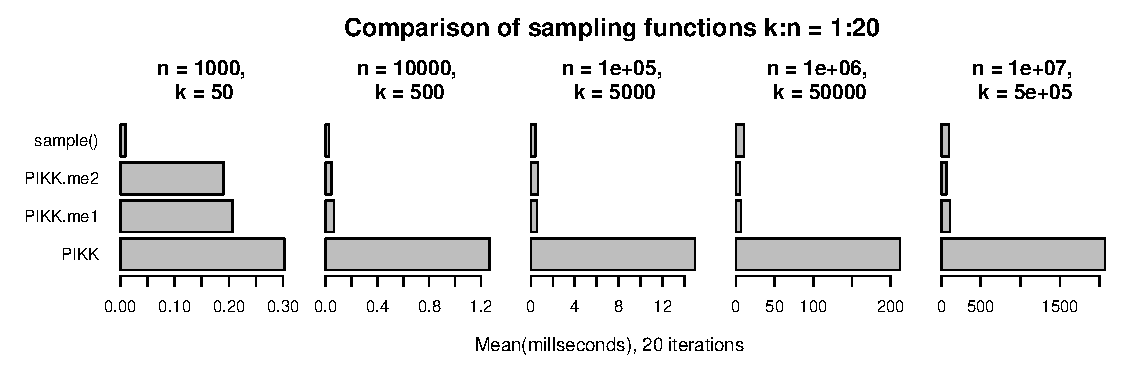
\includegraphics[width=\maxwidth]{figure/plots-1} 
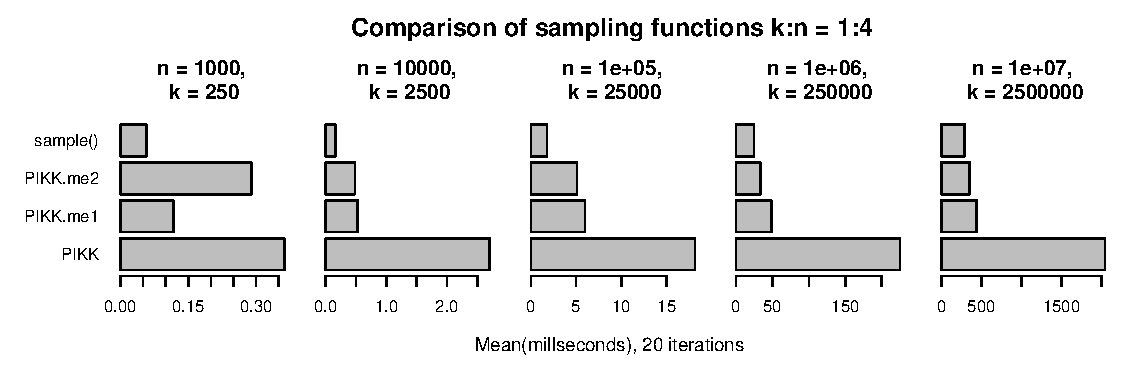
\includegraphics[width=\maxwidth]{figure/plots-2} 
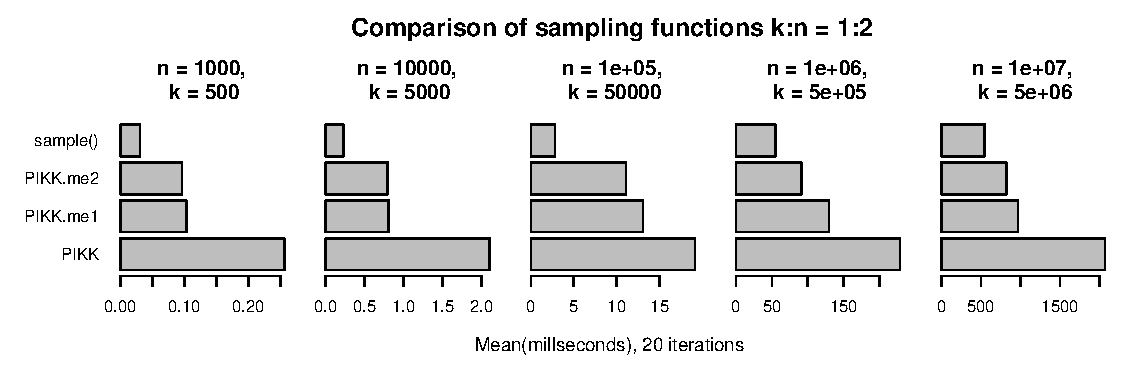
\includegraphics[width=\maxwidth]{figure/plots-3} 
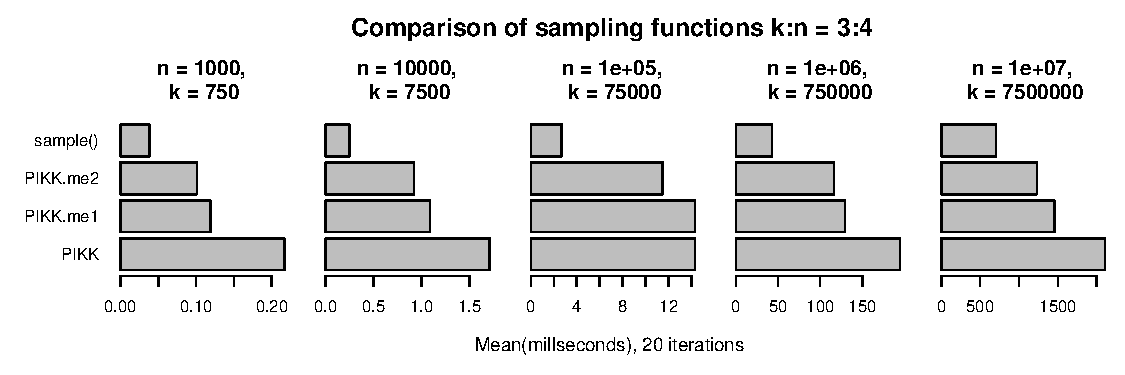
\includegraphics[width=\maxwidth]{figure/plots-4} 

\end{knitrout}


Both of my verions of PIKK are faster than the default version. The second version, \texttt{PIKK.me2} is approximately as fast as \texttt{sample()}, and for some values of \texttt{n}, and \texttt{k}, \texttt{PIKK.me2} is faster than \texttt{sample()}. \texttt{PIKK.me2} gets more efficient as n increases. All methods slow down with ratio of k:n increases. Sample appear to decrease in efficiency as n and k get get large.

\subsection{Extra credit:}

My function \texttt{PIKK.me2} is almost as fast as \texttt{sample()} and qualifies for extra credit because of its speed.






\end{document}
